\documentclass{mscreport}
\usepackage{titlePage}
\usepackage{setspace}
%\usepackage{dtklogos} % this is just used for typesetting \BibTeX, and may thus be removed
%\usepackage[acronym]{glossaries}
\usepackage{csquotes}
\usepackage{tabulary}
\usepackage{booktabs}
\usepackage{algorithm}
\usepackage{algorithmicx}
\usepackage{algpseudocode}
\usepackage{graphicx}
\usepackage{adjustbox}
\usepackage{listings}
\usepackage{url}
\usepackage{hyperref}
\usepackage[normalem]{ulem}
\useunder{\uline}{\ul}{}
\usepackage[title]{appendix}
\usepackage{tocloft}
\usepackage{hanging}
%\usepackage[nottoc]{tocbibind}
%\renewcommand{\contentsname}{\centering Contents} 
%\makeglossaries
\DeclareUrlCommand\UScore{\urlstyle{rm}}
%center the table of contents title
\renewcommand{\contentsname}{\hfill\bfseries\Large Contents\hfill}   
\renewcommand{\cftaftertoctitle}{\hfill}
%center the table of contents title
%\setlength{\parindent}{4em}
%\setlength{\parskip}{1em}
% abbreviations:
%\newacronym{os}{OS}{Operating System}

% Options -> Config -> QuickBuild -> PdfLaTex + Bib(la)tex + PdfLaTex x2 + View pdf

\begin{document}
\pagenumbering{gobble} %diable page numbering until set again
\author{Student Number: 180240438	}
\title{Measuring Adoption of Security Features in the HTTPS Ecosystem}
%\studentname set from titlePage.sty
\supervisor{Simon Bell}
\universitycrestpath{../images/rhuol_logo_2}

\maketitle 


\begin{center}
    {\Large\bfseries Anti-Plagiarism Declaration}
    \vspace{1cm}
\begin{enumerate}

I declare that this assignment is all my own work and that I have acknowledged all quotations from published or unpublished work of other people.  I also declare that I have read the statements on plagiarism in Section 1 of the Regulations Governing Examination and Assessment Offences, and in accordance with these regulations I submit this project report as my own work.

\begin{flushleft}

\includegraphics[scale=0.21]{../images/signature.png} %placeholder for your signature image
\newline
  \begingroup
    \setstretch{2}
    \noindent\textsf{Student Name} \vspace{0.5cm}\\
    \noindent\textsf{26st March 2018}
  \endgroup
  \end{flushleft}

\end{enumerate}
\end{center}

\newpage

\begin{center}
\section*{Acknowledgements}
\end{center}

Thank you coffee.

\newpage

\pagenumbering{roman}
\setcounter{page}{1}
\vspace*{\fill}
\begin{center}
\begin{huge}
Intentionally Blank
\end{huge}
\end{center}
\vspace{\fill}

\newpage

\begin{center}
\section*{Executive Summary}
\end{center}
\addcontentsline{toc}{section}{Executive Summary}

Executive Summary 

\newpage
\begin{center}
\section*{Acronyms}
\end{center}
\addcontentsline{toc}{section}{Acronyms}


\noindent \textbf{CSS} Cascading Style Sheets \par
\noindent \textbf{CORS} Cross-Origin-Request-Sharing \par
\noindent \textbf{CSP} Content Security Policy \par
\vspace{0.5cm}
\noindent \textbf{DOM} Document Object Model \par
\vspace{0.5cm}
\noindent \textbf{FIPS} Federal Information Processing Standards \par
\vspace{0.5cm}
\noindent \textbf{HTML} Hypertext Markup Language \par
\noindent \textbf{HTTP} Hypertext Transfer Protocol \par
\vspace{0.5cm}
\noindent \textbf{MIME} Multipurpose Internet Mail Extensions \par
\vspace{0.5cm}
\noindent \textbf{URI} Uniform Resource Identifier \par
\noindent \textbf{URL} Universal Resource Locator \par
\vspace{0.5cm}
\noindent \textbf{SSL} Secure Socket Layer \par
\vspace{0.5cm}
\noindent \textbf{TLS} Transport Layer Security \par
\vspace{0.5cm}
\noindent \textbf{XSS} Cross-Site Scripting \par

\newpage

\begin{center}
\section*{Glossary}
\end{center}
\addcontentsline{toc}{section}{Glossary}

\begin{hangparas}{.25in}{1}
\textbf{Cascading Style Sheets} is a mechanism by which a web page can be styled by many different aspects such as fonts, colours and spaces. \par
\textbf{Cipher Suite} Defines the implementation of cryptographic primitives and addition information referable via a unique identifier such as \UScore{TLS_ECDHE_RSA_WITH_AES_128_GCM_SHA256} for the use in establishment of SSL/TLS connections \cite{Ristic2017-aj}. \par
\textbf{Cross Origin-Request-Sharing} Is a web browser mechanism for the purpose of allowing a resource to specify the origins allowed to access the resource via the use of HTTP Headers. \par
\textbf{Cross Site Scripting} An injection attack method where scripts are injected into a trusted website for the purpose of performing wanted actions on a user’s online account and or gaining access to sensitive information (e.g. authentication cookies and session identifiers) usually via a web browser. \par
\textbf{Content Security Policy} is a HTTP protocol feature to restrict which resources can be fetched and or executed, such as for the purposes of obtaining content e.g. images, whilst on a specific web page in a web browser. The policy details can be specified in either a HTTP Header or as a meta tag in the html body of a web page. \par
\vspace{0.5cm}
\textbf{Document Object Model} is the web browsers internal representation of an html page as a result of the browser parsing the html \cite{Apple_undated-ay}. \par
\vspace{0.5cm}
\textbf{Federal Information Processing Standards} Are standards for US federal computer systems and are developed by the National Institute of Standards and Technology (NIST) \par
\vspace{0.5cm}
\textbf{Hypertext Markup Language} A standardised language to create documents \cite{Berners-Lee1995-hg} for instructing a web browser how a web page should be rendered/visualised. \par
\textbf{Hypertext Transfer Protocol} A stateless application level protocol \cite{Berners-Lee1996-ji} for the transmission of data (e.g. HTML) typically between a website and a web browser. \par
\vspace{0.5cm}
\textbf{Multipurpose Internet Mail Extensions} is used to announce the intended format of a resource (e.g document or file) \cite{Freed2013-yn}. \par
\vspace{0.5cm}
\textbf{Universal Resource Locator} A specific type of URI that has a scheme (how to access) and a resource (where to access). The most basic form of a URI is as follows \texttt{$<$scheme$>$:$<$scheme-specific-part$>$}. An example URL is \texttt{https://www.example.com} \par
\vspace{0.5cm}
\textbf{Secure Socket Layer} A protocol to establish a secure communications channel mainly used by the HTTP protocol \par
\vspace{0.5cm}
\textbf{Transport Layer Security} A protocol, successor of the SSL protocol, to establish a secure communications channel mainly used by the HTTP protocol \par

\end{hangparas}



\newpage

\addcontentsline{toc}{section}{\listfigurename}
\listoffigures

\newpage
\addcontentsline{toc}{section}{\listtablename}
\listoftables

\newpage

%\printglossary[type=\acronymtype,title=List of Abbreviations,nonumberlist]
%\newpage



\pagenumbering{arabic}
\tableofcontents

\newpage

\section{Introduction}

Describe structure of the introduction

\subsection{Motivation}

Motivation for the project

\subsection{Objectives}

The objectives of this project are:
\begin{itemize}
  \item Objective 1
  \item Objective 2
  \item Objective 3
  \item Objective 4
  \item Objective 5
\end{itemize}  
  
\subsection{Structure of the Report}

Describe structure of the whole report

\newpage

\section{Background Research}

Background research section

\subsection{Background research sub-section 1}

Background research 

\begin{table}[h!]
  \begin{center}
    \caption{Your first table.}
    \label{tab:table1}
    \begin{tabular}{l|c|r} % <-- Alignments: 1st column left, 2nd middle and 3rd right, with vertical lines in between
      \textbf{Value 1} & \textbf{Value 2} & \textbf{Value 3}\\
      $\alpha$ & $\beta$ & $\gamma$ \\
      \hline
      1 & 1110.1 & a\\
      2 & 10.1 & b\\
      3 & 23.113231 & c\\
    \end{tabular}
  \end{center}
\end{table}

\subsection{Sub-section 1}

Although Google has lately employed Google Play Protect \cite{GooglePlayP2017},   which is a system that continuously scans the user's mobile to keep him or her away from malicious applications and tries to improve the user's mobile security, malicioussssss developers always finds ways and means to bypass both the security mechanisms employed by mobile anti-malware software and furthermore, Android OS security mechanisms. In \cite{SuarezTangil2014}, Suarez-Tangil \textit{et al.} presents a thorough study on the evolution of malware for smart devices, some characteristics of the current malware and concludes with a survey on detection techniques to prevent malware on smart devices. When it comes to the current security models, the researchers highlight three different fundamentals in which are mainly divided between the security of the application market, the security of the operating system and the third fundamental is the overview proposals of latest security mechanisms with specialisation to the Android malware. The researchers continue their study by highlighting different malware characterizations starting from attack goals and behaviour, continuing to the distribution of the malware and finalizing to privilege acquisition. In their survey, Suarez-Tangil \textit{et al.} presents the main attack goals, the associated motives behind the malware and exhibited behaviour for malware in smart devices. \newline

\begin{figure}[h!]
\begin{center}
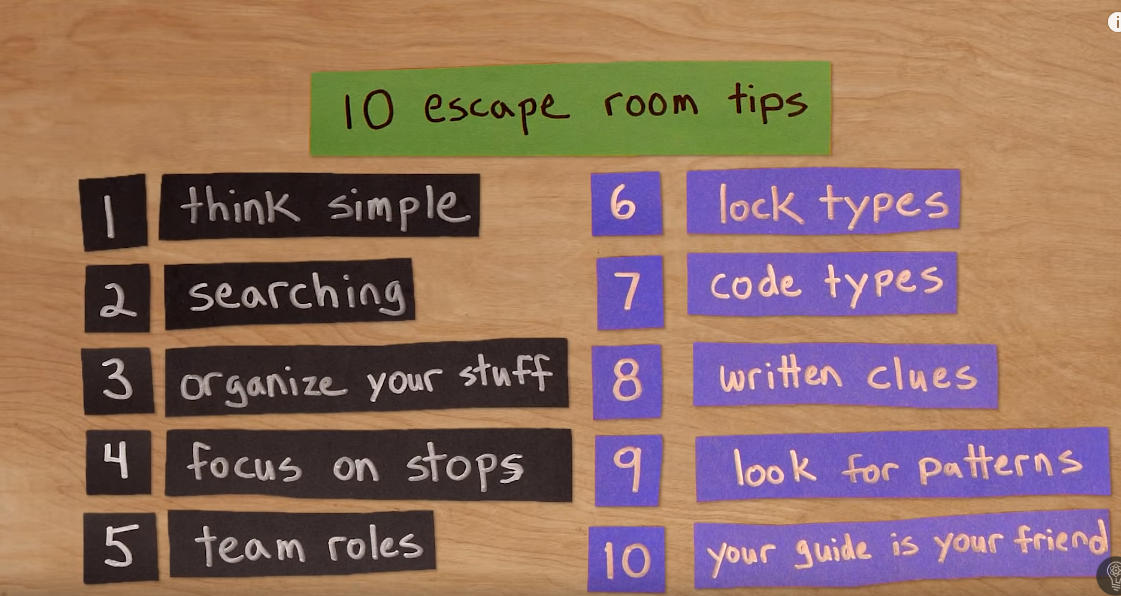
\includegraphics[scale=0.4]{../images/figure_1.png} 
\caption{Different malware characterizations in smart devices \cite{SuarezTangil2014}}
\label{Figure 1: Different malware characterizations in smart devices }
\end{center}
\end{figure}

\clearpage

\section{Proposed Solution}

Section to describe the work being proposed.

\subsection{Sub-section 1}

Sub-section 1 of the proposed solution.

\subsubsection{Sub-subsection 1}

Sub-subsection 1 of the proposed solution.

\begin{algorithm}
\caption{Algorithm 1}\label{euclid}
\begin{algorithmic}
\If {$A$ intersect with $B$ is $True$}
	\State {\textit{A intersects}}
\ElsIf{$A$ = $C$}
	\State {\textit{A equals C}}
\Else \State {\textit{A does not intersect with B and is not equal to C}}
\EndIf   
\end{algorithmic}
\end{algorithm}

\newpage

\section{Evaluation}

Section to describe the testing done.  

\subsection{Sub-section 1}

Sub-section 1 of the evaluation section.

\subsection{Comparison to Current Work}

Compare the work done with other work proposed by other researchers.
\clearpage

\section{Conclusions}

Conclusion section.

\subsection{Limitations}

The solution being proposed has the following limitations:
\begin{itemize}
 \item Limitation 1
 \item Limitation 2
 \item Limitation 3
\end{itemize}

\subsection{Future Work}

Any future work to be done.

\subsection{Conclusion}

Final conclusion and illustrating the objectives met are the following: 
\begin{itemize}
	\item Objective 1
	\item Objective 2
	\item Objective 3
	\item Objective 4
	\item Objective 5
\end{itemize}

Final summary of each chapter.

\newpage

\bibliographystyle{IEEEtran}
%Mendeley automatically generatex BibTex file to be included
\bibliography{IEEEabrv,library}

\newpage

\begin{appendices}
\section{Title of Appendix}

Some text.

\end{appendices}

\end{document}
